% ----------------------------------------------------------------------------------------------------------------------
%       MPI PRACTISE
% ----------------------------------------------------------------------------------------------------------------------

\documentclass[onecolumn]{article}
\usepackage[utf8]{inputenc}   %con esto, voy a permitir los acentos sin menester del codigo
\usepackage[english]{babel}
%%%%%%%%%%%%%%%%%%%%%%%%%%%%%%%%%%%%%%%%%%%
\usepackage{graphicx,epsfig}
\usepackage{mathtools}
\usepackage{amsfonts,amsmath,amssymb,amsthm} 
\usepackage{relsize}
\usepackage{dcolumn}
\usepackage{array}
\usepackage{graphicx}
\usepackage{ulem}
\usepackage{subfig}
\usepackage{sidecap}
%\usepackage{wrapfig}
\usepackage{lipsum}
\usepackage{hyperref}
\usepackage{floatrow}
\usepackage{fancyhdr}
\usepackage{bm} %bold math symbols
\usepackage{hhline}

%%%%%%%%%%%%%%%%%%%%%%%%%%%%%%%%%%%%%%%%%%%
\newfloatcommand{capbtabbox}{table}[][\FBwidth]
\renewcommand{\vec}[1]{\mathbf{#1}} 
\renewcommand{\it}[1]{\textit{#1}}
\renewcommand{\d}{\text{d}}

\begin{document}

% --- Configurar la pagina ---------------------
\pagestyle{fancy}
\lhead{\bf Memoria EIA}
\rhead{Máster en Modelización Atomística y Multiescala}
%\lfoot{ }
\rfoot{Barcelona, Marzo 2017}
% ----------------------------------------------


\title{Implementación de un código de Dinámica Molecular en serie y en paralelo usando el módulo MPI}
\author{Oscar Fajardo, Xavier Marugán, Xabier Méndez, Alberto Pla,\\ Sergi Roca, Sotiris Samatas, Elena Sesé y Lorena Vega}
\date{Jueves 30 de Marzo}

\maketitle

\section{Initialisation of the system}


\section{Cálculo de Fuerzas: Lennard-Jones}
Hemos implementado la interacción de Lennard-Jones para calcular las fuerzas entre pares de partículas.

\begin{equation} \label{eq:1}
 \vec{F}_{LJ} (r) = 24 \epsilon  \left(2 \frac{{\sigma}^{12}}{r^{13}} -  \frac{{\sigma}^{6}}{r^{7}}\right)\hat{r}
\end{equation}

donde $\epsilon = 1$ y $\sigma = 1$.


El cómputo de las fuerzas en serie se reduce a calcular la distancia entre los pares de partículas, aplicando condiciones periódicas de contorno, y usar la Eq. (\ref{eq:1}) para obtener el valor de la fuerza que recibe cada partícula. 

Para realizar el algoritmo en paralelo hemos divido las partículas por procesadores, lo que se conoce como \textit{Atom decomposition algorithm}. Es decir, hemos repartido un número igual de partículas para cada procesador, Fig \ref{interaction_mat1}. Cuando el número de partículas no sea divisible entre el número de procesadores, el último procesador se quedará con las partículas de más, hasta la última. 

\begin{figure}[ht]
\begin{equation*}
G_{i,j}=\begin{pmatrix}
\bullet  & \bullet & \bullet &\bullet  &\bullet  & \bullet & \bullet &\bullet \\ 
 \bullet&\bullet  &  \bullet& \bullet & \bullet & \bullet & \bullet &\bullet \\
 \bigtriangleup&\bigtriangleup  &  \bigtriangleup& \bigtriangleup & \bigtriangleup & \bigtriangleup & \bigtriangleup &\bigtriangleup \\
 \bigtriangleup&\bigtriangleup  &  \bigtriangleup& \bigtriangleup & \bigtriangleup & \bigtriangleup & \bigtriangleup &\bigtriangleup \\
 \diamond & \diamond  &  \diamond&  \diamond & \diamond &  \diamond &  \diamond & \diamond \\
 \diamond & \diamond  &  \diamond&  \diamond & \diamond &  \diamond &  \diamond & \diamond \\
 \star & \star  &  \star&  \star & \star &  \star &  \star & \star \\
 \star & \star  &  \star&  \star & \star &  \star &  \star & \star
 \end{pmatrix}
\end{equation*}
\caption{Separación de partículas por procesador. En este caso tenemos 8 partículas y 4 procesadores. Cada símbolo representa las interacciones que calculará cada procesador. }
\label{interaction_mat1}
\end{figure}

\subsection{Método 1: \textit{Atom decomposition} algorithm}

Trabajando con N partículas y 3 dimensiones, cada \textit{worker} calculará la interacción entre el número de partículas que se le han asignado y las N partículas del sistema. Ésta será la información que cada \textit{worker} le pase al procesador master, que finalmente obtendrá una matriz de fuerzas NxNx3, $\vec{G}_{ij}$. Esta matriz contiene la fuerza de cada partícula del sistema con todas las restantes. Una vez toda la información esté en el master, hay que sumar, en nuestro caso el segundo índice, para obtener la fuerza que cada partícula recibe por acción del resto, obteniendo así una matriz de fuerzas Nx3, $\vec{F}_{k}$. A continuación, se procederá a enviar esta matriz a todos los \textit{workers}. El proceso finaliza cuando todos los \textit{workers} reciben la matriz entera actualizada.

\begin{figure}[ht]
\begin{center}
\includegraphics[width=0.6\textwidth, angle=-90]{time_particlesE.eps}
\caption{Tiempo de cálculo de las fuerzas, de la comunicación entre procesadores y de la suma de interacciones en función de las partículas del sistema, fijando 8 procesadores, según el método 1.}
\label{elena_1}
\end{center}
\end{figure}

Esquemáticamente, el algoritmo utilizado es:

\begin{enumerate}
    \item Separación de partículas por procesadores.
    
    \item Envío de cada trozo de la matriz $\vec{G}_{ij}$ de los \textit{workers} al master.
    \item El master recibe toda la matriz $\vec{G}_{ij}$.
    \item El master calcula la fuerza total por partícula $\vec{F}_{k}$ (Eq. \ref{eq:1}).
    \item Envío de la matriz $\vec{F}_{k}$ desde el master a todos los demás procesadores.
    \item Todos los procesadores reciben la matriz $\vec{F}_{k}$ del master.
\end{enumerate}



\begin{figure}[ht]
\begin{center}
\includegraphics[width=0.6\textwidth, angle=-90]{time_procE.eps}
\caption{Tiempo de cálculo de las fuerzas, de la comunicación entre procesadores y de la suma de interacciones en función del número de procesadores, fijando el número de partículas a 10000, según el método 1.}
\label{elena_2}
\end{center}
\end{figure}

Observando la Fig. \ref{elena_1} y como se esperaba, el tiempo de todos los procesos que hace el programa en paralelo aumenta con el número de partículas.

El aumento de partículas se traduce en un aumento de pares entre los cuales calcular la fuerza de interacción. Por eso el cálculo de las fuerzas se ralentiza. Del mismo modo, la comunicación entre procesadores es más lenta porque las matrices $\vec{G}_{ij}$ que tienen que enviar y recibir son de mayor tamaño. 

El proceso que menos afectado se ve por el aumento de partículas es la suma de la fuerza total por partícula. 

En la Fig. \ref{elena_2} se ve la variación del tiempo de computación de los distintos procesos que realiza el programa en función del número de procesadores usados para computar en paralelo. 

El tiempo de computación de las fuerzas es el proceso que lleva más tiempo.  Se observa también que repartir el cálculo entre más procesadores disminuye el tiempo de computación. Es más óptimo por tanto dividir el trabajo entre distintos procesadores, como cabía esperar.  

El tiempo que lleva calcular la fuerza total por partícula se mantiene constante porque es un proceso que se hace en serie y, por tanto, únicamente depende del número de partículas, aquí fijo.

La comunicación es más rápida cuando hay menos procesadores entre los que pasar información. No obstante, a partir de 6 procesadores aproximadamente, el tiempo de computación se mantiene constante. Podemos concluir que la comunicación entre procesadores se ve mucho más afectada por la cantidad de datos que se tengan que enviar y recibir que no por el número de procesadores que se usen.






\subsection{Método 2: \textit{Atom decomposition} algorithm with \textit{Newton's second law}}



Con el \textit{Atom decomposition algorithm} se puede aplicar la tercera ley de Newton, por la cual $\vec{G}_{ij}=-\vec{G}_{ji}$. y por lo tanto no hace falta calcular todos los pares de partículas sino solamente la mitad. 

En un programa en serie esto es fácilmente implementable ya que solo se calcula la diagonal superior de la matriz de interacciones $\vec{F}_{ij}$. En el caso del programa en paralelo, al separar la matriz de interacciones por partículas, es decir, cada procesador solo calcula la interacción entre unas pocas partículas con todas las demás como se muestra en la Fig. \ref{interaction_mat2}, la forma de calcular la mitad de las interacciones tiene que hacerse de una forma un tanto diferente. Para que todos los procesadores tengan un numero igual o parecido de interacciones que calcular solo se calcularan los coeficientes de matriz en los que $i+j$ es par cuando $j>i$ y los coeficientes donde $i+j$ es impar cuando $j<i$.

\begin{figure}[ht]
\begin{equation*}
  G_{ij} = \begin{pmatrix}
\circ  & \circ & \bullet & \circ & \bullet\\ 
\bullet & \circ & \circ &\bullet  & \circ\\ 
\circ & \bullet & \circ & \circ &\bullet \\ 
\bullet & \circ & \bullet &\circ  &\circ \\ 
\circ &\bullet  & \circ &\bullet  & \circ
\end{pmatrix}
\end{equation*}
\caption{Matriz de interacciones entre todas las partículas. Solo se calculan los coeficientes en los que $i+j$ es par cuando $j>i$ y los coeficientes donde $i+j$ es impar cuando $j<i$.}
\label{interaction_mat2}
\end{figure}

\begin{figure}[ht]
\begin{center}
\includegraphics[width=0.6\textwidth, angle=-90]{forces_proc1.eps}
\caption{Cálculo de las fuerzas con el método 2. Número de partículas = 10000.}
\label{xabi_1}
\end{center}
\end{figure}

Por consiguiente, cada procesador calculará un número predeterminado de filas de la matriz de interacción $\vec{F}_{ij}$ de la Fig. \ref{interaction_mat2}. Una vez calculado, cada procesador mandará su trozo de la matriz al master y éste calculará la fuerza total que siente cada partícula de la siguiente manera:

\begin{equation}
    F_k = \sum_{j=1}^N G_{k,j} - \sum_{i=1}^N G_{i,k}
\end{equation}
\label{sum}

dónde $F_k$ es la fuerza total que siente cada partícula.

Por último, ahora que el master tiene la fuerza que siente cada partícula tiene que mandar esta matriz a todos los demás procesadores. Resumiendo, la paralelización se ha hecho de la siguiente manera:

\begin{enumerate}
    \item Separación de partículas por procesadores.
    \item Cálculo de la mitad de términos de la matriz de interacciones $\vec{G}_{ij}$ como en la Fig. \ref{interaction_mat2}. Cada procesador calculara un número de filas.
    \item Envío de cada trozo de la matriz $\vec{G}_{ij}$ al master.
    \item El master recibe toda la matriz $\vec{G}_{ij}$.
    \item El master calcula la fuerza total por partícula $\vec{F}_{k}$ (Eq. \ref{sum}).
    \item Envio de la matriz $\vec{F}_{k}$ desde el master a todos los demás procesadores
    \item Todos los procesadores reciben la matriz $\vec{F}_{k}$ del master.
\end{enumerate}

\begin{figure}[ht]
\begin{center}
\includegraphics[width=0.6\textwidth, angle=-90]{forces_part1.eps}
\caption{Cálculo de fuerzas con diferente número de partículas con el método 2. Número de procesadores = 8.}
\label{xabi_3}
\end{center}
\end{figure}



Como se puede observar en la Fig. \ref{xabi_1}, vemos que el proceso de calcular la fuerza total por partícula mediante la suma de la Eq. \ref{sum} (5º paso) es el proceso que más tiempo de computación lleva. Esto se debe a que este proceso solo lo hace el master y por lo tanto, se hace en serie. Por otro lado, vemos que el tiempo de comunicación se mantiene constante casi para cualquier número de procesadores y que el tiempo de cálculo de fuerzas decrece lentamente con muchos procesadores por lo que por mucho que añadamos muchos más procesadores que 24 no conseguiremos disminuir mucho el tiempo.

En la linea verde de la Fig. \ref{xabi_2} podemos ver que el tiempo total utilizando este método decrece con el número de procesadores pero a partir de 15 se mantiene casi constante, es decir, 15 procesadores sería el número óptimo de procesadores para éste tipo de paralelización.


Si se analiza el tiempo de computación respecto al número de partículas (Fig. \ref{xabi_3}) se puede observar que el tiempo de cálculo de fuerzas será más grande que el de comunicación entre procesadores para un número de partículas muy grande. Aún así, el tiempo de cálculo de la suma de fuerzas sigue siendo mucho más grande que los otros dos y és lo que hace que este método sea muy lento. Por esa razón, a continuación se propone otro método para reducir el tiempo de cálculo del proceso de la suma de la fuerza.

\subsection{Método 3: Full parallelization of \textit{Atom decomposition} algorithm with \textit{Newton's second law}}
Para este método de paralelización se han seguido los mismos pasos que en el método 2 hasta el 4º paso. Después, en este caso, una vez el master tiene la matriz de interacciones $\vec{G}_{ij}$ entera, la envía a todos los demás procesadores. Ahora, cada procesador calcula la fuerza total de las partículas que se le han asignado por lo que cada procesador tendrá un trozo de la matriz $\vec{F}_{k}$. Para juntar esta matriz, cada procesador tiene que enviarla el master y una vez que el master tenga la matriz entera volverla a enviar a todos los procesadores. En resumidas cuentas, el método quedaría de la siguiente manera:
\begin{figure}[h]
\begin{center}
\includegraphics[width=0.6\textwidth, angle=-90]{forces_proc2.eps}
\caption{Cálculo de fuerzas con diferente número de procesadores con el método 3. Número de partículas = 10000.}
\label{xabi_5}
\end{center}
\end{figure}

\begin{figure}[h]
\begin{center}
\includegraphics[width=0.6\textwidth, angle=-90]{forces_part2.eps}
\caption{Cálculo de fuerzas con diferente número de partículas con el método 3. Número de procesadores = 8.}
\label{xabi_4}
\end{center}
\end{figure}


\begin{enumerate}
    \item Separación de partículas por procesadores.
    \item Cálculo de la mitad de términos de la matriz de interacciones $\vec{G}_{ij}$ como en la Fig. \ref{interaction_mat2}. Cada procesador calculara un número de filas.
    \item Envio de cada trozo de la matriz $\vec{G}_{ij}$ al master.
    \item El master recive toda la matriz $\vec{F}_{ij}$.
    \item El master envía la matriz $\vec{G}_{ij}$ entera a todos los demás procesadores.
    \item Todos los procesadores reciben la matriz $\vec{G}_{ij}$ del master.
    \item Cada procesador calcula la fuerza total sobre las partículas que le hayan sido asignadas en el paso 1 calculando así un trozo de la matriz $\vec{F}_{k}$.
    \item Envío de cada trozo de la matriz $\vec{F}_{k}$ al master.
    \item El master recibe toda la matriz $\vec{F}_{k}$.
    \item El master envía la matriz $\vec{F}_{k}$ entera a todos los demás procesadores.
    \item Todos los procesadores reciben la matriz $\vec{F}_{k}$ del master.
\end{enumerate}

Como se puede observar en la Fig. \ref{xabi_5}, vemos que comparado con los 15 segundos que tardaba en el método 2 (Fig. \ref{xabi_1}, el proceso de sumar las fuerzas ha disminuido en tiempo considerablemente. Además, como la suma está paralelizada vemos que disminuye con el número de procesadores utilizados. Hay que destacar que este método es muy complejo a la hora de implementar la comunicación entre procesadores y es por eso que no se ha conseguido un código que funcione siempre. Por esa razón, solo se han podido utilizar un máximo de 8 procesadores.

También podemos ver que el tiempo de comunicación es ligeramente mayor en el método 3 (Fig. \ref{xabi_5}) que en método 2 (Fig. \ref{xabi_1}) pero como el tiempo de suma es muchísimo más pequeño este método es mucho más rápido, como se puede observar en la linea azul de la Fig. \ref{xabi_2}.

Analizando el tiempo de computación según el número de partículas se puede ver en la Fig. \ref{xabi_4} que el tiempo de suma ha decrecido considerablemente comparándolo con el de la Fig. \ref{xabi_3}. Cabe destacar que los cálculos a partir del número de partículas igual a 9000 no fueron realizados correctamente y por lo tanto esos puntos no se deben tomar en cuenta.

Para terminar, en la Fig. \ref{xabielena} se puede observar que el método 3 es muchísimo mejor que el 2 y que para pocas partículas es tan eficiente como el código en serie aunque hay que resaltar que nunca mejora el tiempo del código en serio. 

\subsection{Comparación de los métodos y conclusiones}

En todos los métodos en paralelo, el tiempo de computación disminuye al aumentar los procesadores. Los métodos 2 y 3 siempre son más lentos que aplicar el algoritmo en serie. Esto se debe a que al realizar la suma de las fuerzas el tiempo computacional es mucho más alto que en el método 1, aunque podría ser un problema de diferentes implementaciones de la suma. La única diferencia está en el método 1. Si bien para pocos procesadores el algoritmo en serie sigue siendo más rápido, a partir de 7 procesadores esta tendencia se invierte, tal y como se ve en la Fig. \ref{xabi_2}.

\begin{figure}[h]
\begin{center}
\includegraphics[width=0.6\textwidth, angle=-90]{forces_proc3.eps}
\caption{Cálculo de fuerzas con diferentes procesadores y diferentes métodos de paralelización. Número de partículas = 10000.}
\label{xabi_2}
\end{center}
\end{figure}

\begin{figure}[h]
\begin{center}
\includegraphics[width=0.6\textwidth, angle=-90]{time_particlesEX.eps}
\caption{Cálculo de fuerzas con distinto número de partículas y diferentes métodos de paralelización. Número de procesadores = 8. }
\label{xabielena}
\end{center}
\end{figure}


También se puede apreciar en la Fig. \ref{xabi_2} que el hecho de calcular las fuerzas en paralelo (método 3) disminuye mucho el tiempo de computación total comparando con el método 2. Aún así, nunca se llega a tiempos tan bajos como los del método 1. En un futuro se podría intentar paralelizar las fuerzas en el método 1 para así conseguir un código todavía más eficiente.

En el caso de la Fig. \ref{xabielena}, el tiempo de computación aumenta con el número de partículas. Como el número de procesadores es 8, el método 1 es más rápido que el algoritmo en serie, independientemente del número de partículas.  Igual que en la Fig. \ref{xabi_2}, los métodos 2 y 3 son mucho más lentos. 

En conclusión, a la hora de paralelizar el código para optimizar el tiempo podemos ver que el único método capaz de superar en velocidad al código en serie es el método 1 aunque puede que para sistemas con muchísimas más partículas el método 3 implementado de manera correcta consiga superar esta velocidad.

Por último, destacar que hemos tenido muchos problemas con las funciones de MPI a la hora de tratar con matrices de tamaño muy grande. Sobretodo, estos problemas se acentúan cuando hay muchos envíos en un mismo código (como es el caso del método 3). Nos hemos dado cuenta de que no teníamos las herramientas de MPI necesarias para solucionar este tipo de problemas.



\section{Integrador de Euler}

Una de las principales partes de una código de dinámica molecular son los integradores de las ecuaciones de movimiento,
aquellos que permiten la propia dinámica.

Para hacer un buen código de dinámica molecular, es menester elegir correctamente qué integrador se va a usar en la simulación.
En esta sección se va a explicar el algoritmo de Euler explícito, uno de los más sencillos que se pueden implementar.

El algoritmo de Euler discretiza e integra las ecuaciones de movimiento Newton, \eqref{eq:newton}, con tal de obtener la trayectoria de las partículas
del sistema simulado.

\begin{equation}\label{eq:newton}
\frac{\d\vec{r_k}}{\d t} = \vec{v_k}\hspace{2cm} \frac{\d\vec{p_k}}{\d t} = \vec{F_k} .
\end{equation}

Dado que se trata de una dinámica molecular, el integrador implementará la actualización de las posiciones y la de las velocidades
a cada paso de tiempo, siguiendo las ecuaciones \eqref{eq:r_euler} y \eqref{eq:v_euler},
\begin{equation}\label{eq:r_euler} 
\vec{r_k}(t+\Delta t) = \vec{r_k}(t) + \vec{v_k}(t)\Delta t + \frac{1}{2m_k}\vec{F_k}(t)\Delta t^2 ,
\end{equation}

\begin{equation}\label{eq:v_euler} 
\vec{v_k}(t+\Delta t) = \vec{v_k}(t) + \frac{1}{m_k}\vec{F_k}(t)\Delta t .
\end{equation}

No obstante, este integrador presenta un problema severo. Dicho problema es la falta de simetría bajo una transformación temporal inversa para $\Delta t$ 
suficientemente grandes. Esto implica que si se quiere implementar un buen algoritmo integrador, habría que tomar pasos de tiempo infinitesimalmente pequeños
al usar el integrador de Euler.

La implementación numérica de este método en un código de DM es sencilla. En cada paso de tiempo, una vez las fuerzas que actúan sobre cada partícula hayan sido
calculadas, se añade este algoritmo para calcular las nuevas posiciones y velocidades.

\subsection{Código en paralelo}
 
 El método usado para paralelizar las dos subrutinas que he implementado, los integradores para las posiciones y para las velocidades, ha sido la herramienta MPI para
 Fortran90.
 
 Con tal de paralelizar el cálculo del update de posiciones y velocidades, he elegido dividir los vectores según el índice correspondiente al número de partículas, i.e.,
 que cada procesador ejecute el cálculo de un segmento de partículas, $[k , k + \delta k]$. El número de partículas que entre en cada procesador vendrá dado por el número
 de procesadores y el número de partículas, e.g, en el caso de 12 partículas y 4 procesadores, cada uno ejecutará los cálculos para 3 partículas.
 
 Una vez cada procesador ha calculado su correspondiente segmento del vector, lo envían al Master (procesador 0), el cual hace un \textit{merge} de todos los segmentos
 con tal de obtener el vector entero de posiciones y velocidades ya actualizado a ese instante de tiempo. Cuando todo el vector está ya actualizado, el Master vuelve a mandar
 el vector a todos los procesadores, consiguiendo así que todos ellos tengan toda la información actualizada.
 
 Para enviar datos entre procesadores, he usado la subrutina del módulo `mpif.h' MPI$\_$ISEND. Una vez los datos han sido enviados, antes de ser recibidos, he implementado
 una barrier, MPI$\_$BARRIER, con tal de esperar a que todos los procesadores hallan enviado su sección del vector y evitar fallos en la comunicación. Cuando la barrera ya ha sido
 superada, los destinatarios reciben los datos con un MPI$\_$RECV, seguido también por una barrera que sólo sea superada una vez todos los destinatarios hayan recibido la información.
 
 Para testear la paralelización, he estudiado la dependencia del tiempo de ejecución de mis subrutinas (posiciones y velocidades por Euler) en función del número de procesadores
 y del número de partículas tratadas. Como se puede ver en los resultados mostrados en la \autoref{fig:posiciones_euler}, la paralelización no ha sido efectuada de modo eficiente,
 pues cuantos más procesadores, más lenta es la ejecución. El mismo comportamiento ha sido observado para el caso del integrador de las velocidades.
 
 \begin{figure}[h!]
	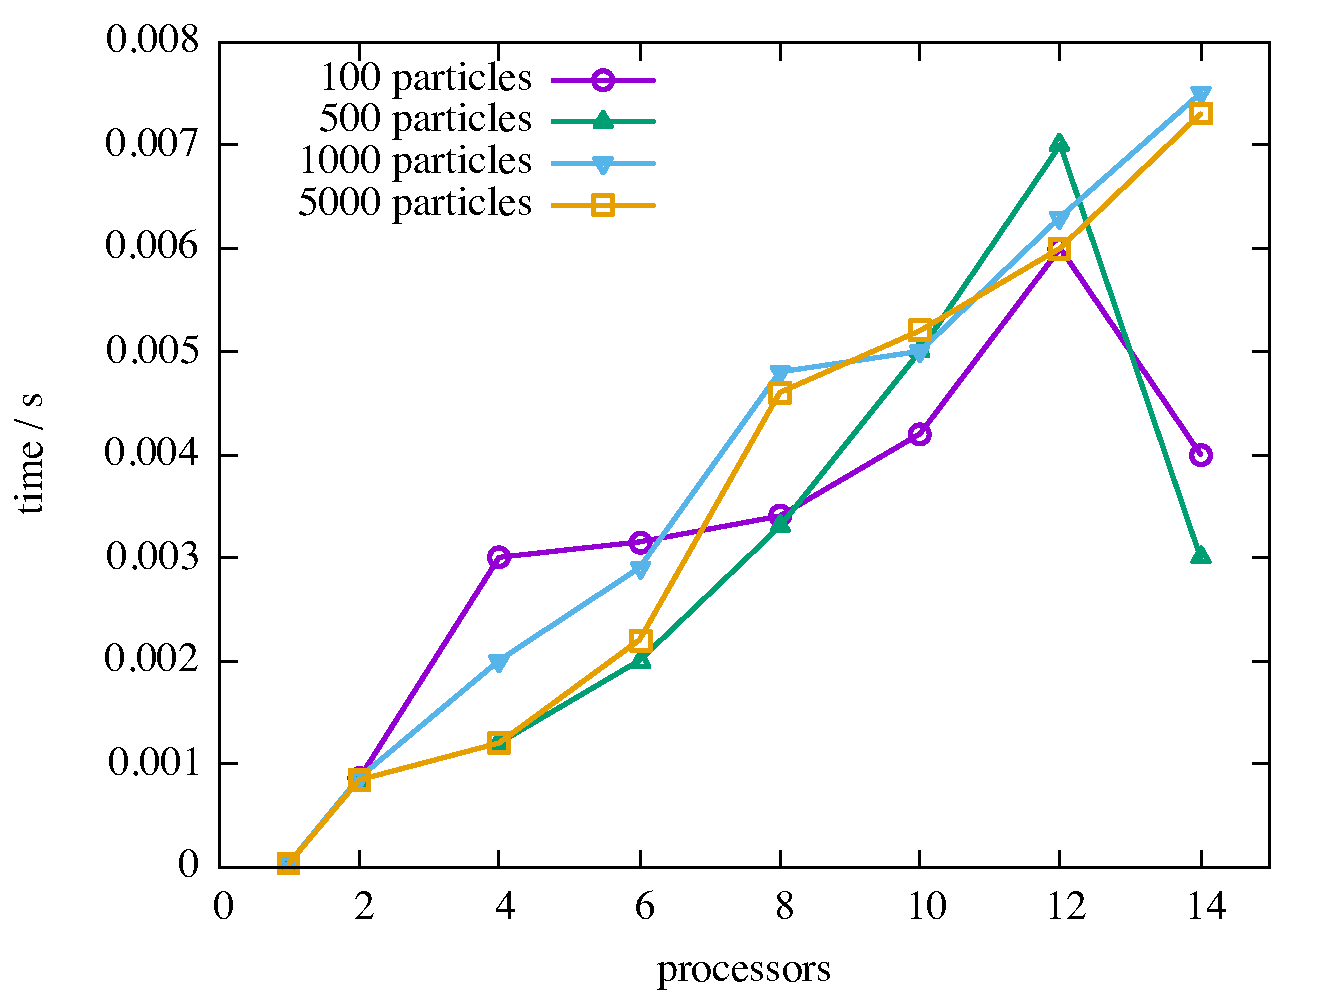
\includegraphics[scale=0.5]{scalate_euler.pdf}
	\caption{Dependencia del tiempo de ejecución del integrador Euler para las posiciones con el número de procesadores y partículas.}
	\label{fig:posiciones_euler}
\end{figure}

	También se puede observar en la misma figura que el número de partículas tratadas tampoco influye significativamente en el tiempo de ejecución. Todo ello lleva a pensar que el método
	usado no ha sido el óptimo, y que la paralelización efectuada no ha servido para acelerar el código. Un posible motivo es la simplicidad de las subrutinas, que sólo consistían en un
	único bucle que recorría todo el vector de posiciones. Bucles de esta índole no son lentos, y escalan correctamente, mientras que el hecho de implementar la comunicación entre los procesadores
	relentiza el código. Cuantos más procesadores, más comunicaciones habrá, y más aumenta el tiempo de ejecución, tal y como se muestra en la \autoref{fig:posiciones_euler}.

\section{Integrador Velocity Verlet}

El segundo integrador usado en el código es velocity Verlet y se aplica usando las siguientes expresiones dependiendo de la variable a integrar:

\begin{equation}
\vec{r}(t+\Delta t) = \vec{r}(t) + \vec{v}(t)\Delta t + \frac{\vec{F}(t)}{2m}\Delta t^2 ,
\end{equation}

\begin{equation}
\vec{v}(t+\Delta t) = \vec{v}(t) + \left( \vec{F}(t)  + \vec{F}(t+\Delta t)\right) \frac{\Delta t}{2m} .
\end{equation}

 \begin{figure}[h!]
	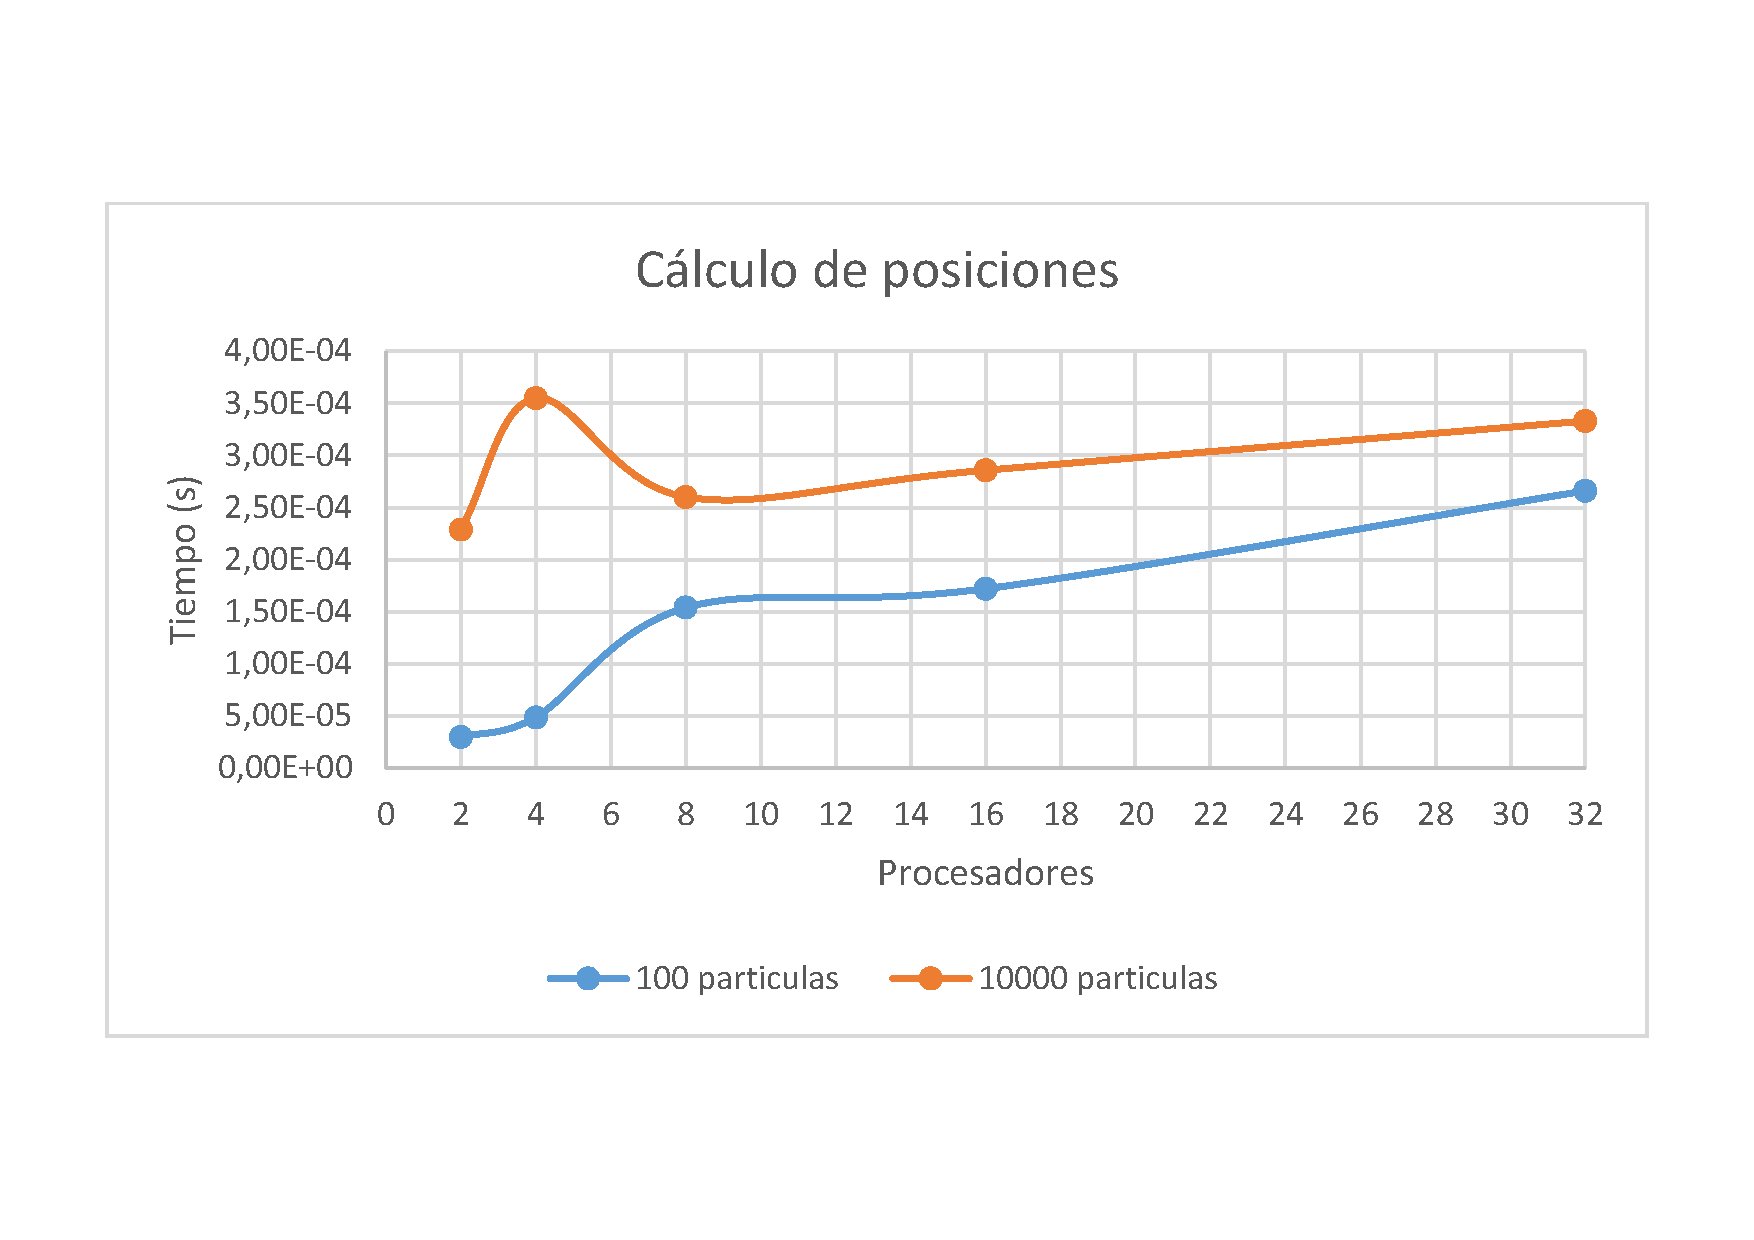
\includegraphics[scale=0.4]{posiciones_verlet.pdf}
	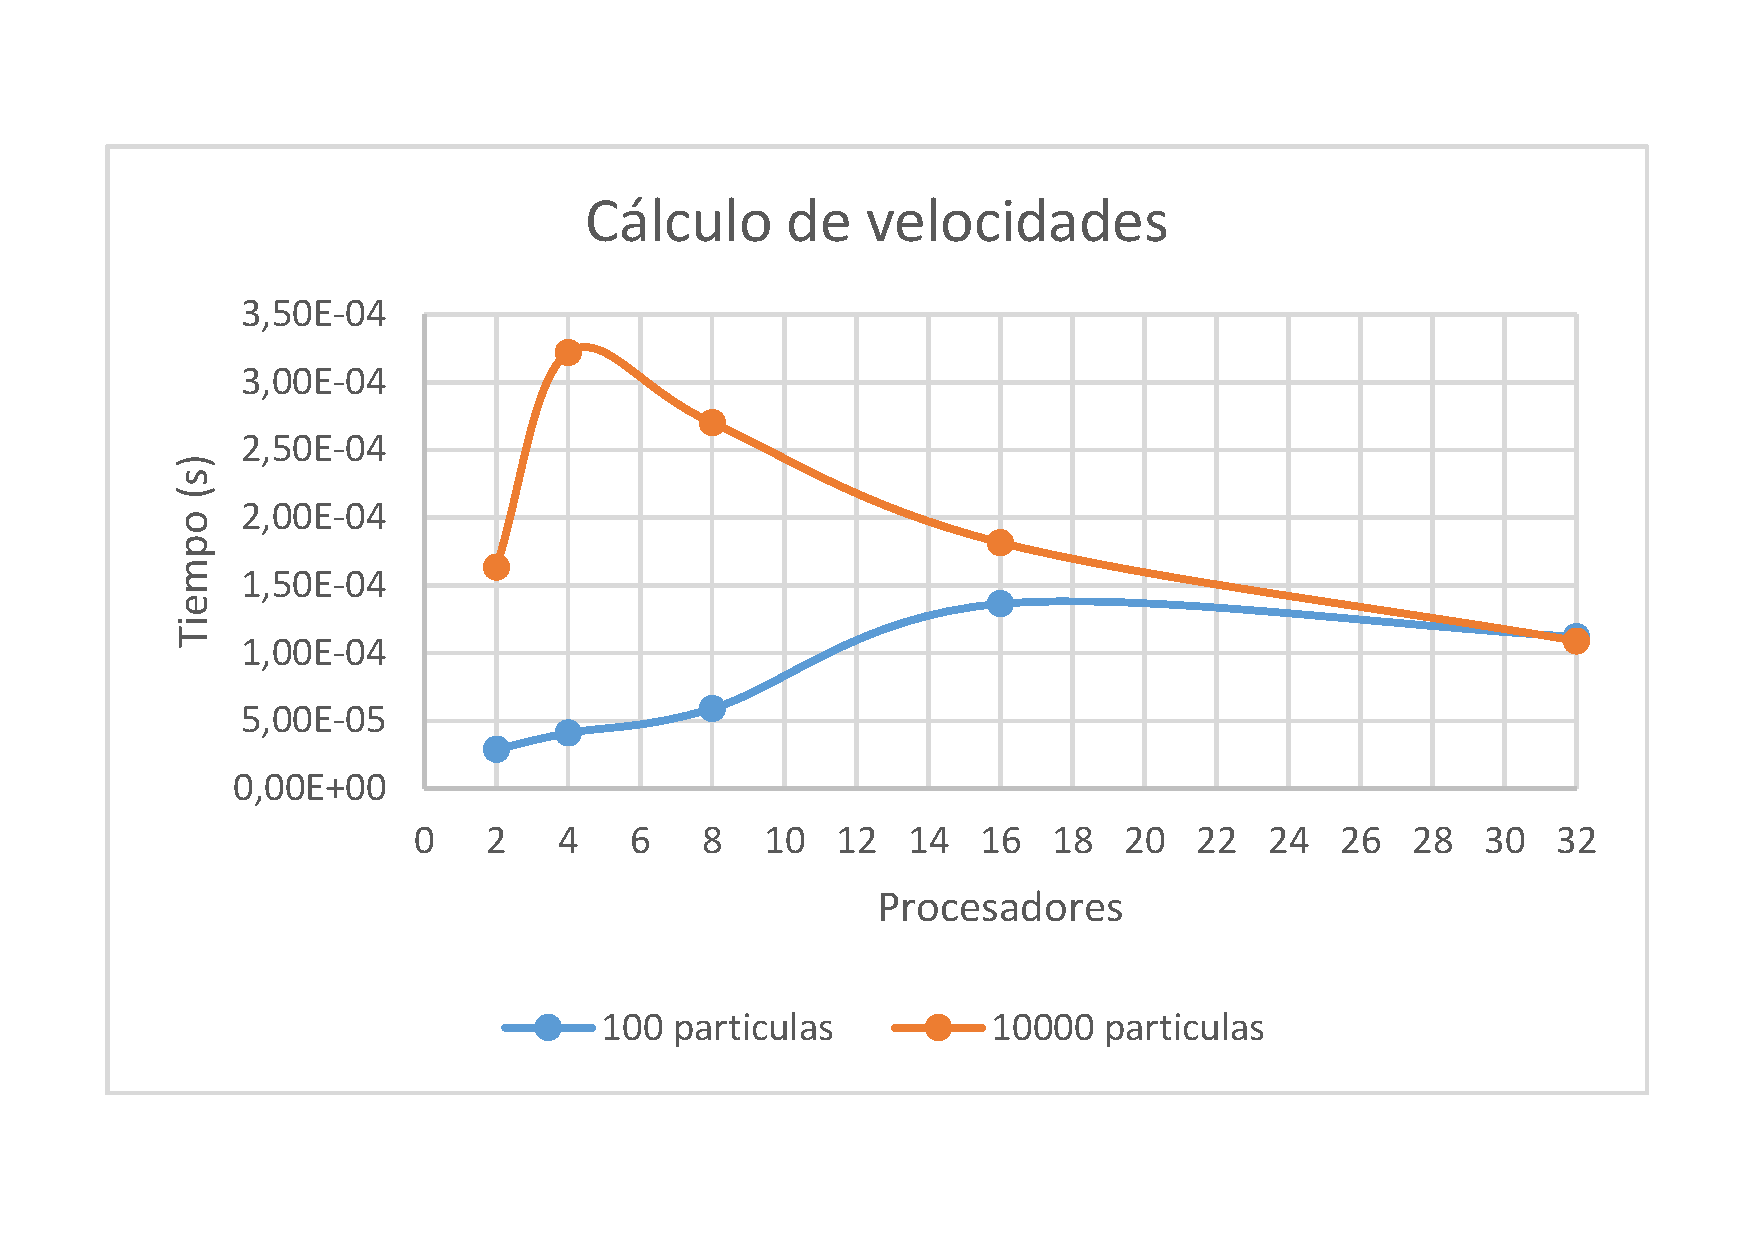
\includegraphics[scale=0.4]{velocidades_verlet.pdf}
	\caption{Dependencia del tiempo de ejecución del integrador Verlet para las posiciones y velocidades con el número de procesadores y partículas.}
\end{figure}

Para calcular las posiciones se usa exactamente la expresión de Velocity Verlet pero para las velocidades está estructurado en dos partes. Primero se calcula la velocidad en el paso de tiempo actual, luego se calculan las fuerzas para actualizar la aceleración de las partículas y finalmente, con la nueva aceleración, se calcula el término a tiempo posterior. El programa tiene esta estructura para no tener que guardar la aceleración en el tiempo anterior para cada partícula, lo que reduce la memoria que necesita el programa.

Al realizar el cálculo en paralelo primero se realiza una parte del cálculo en cada uno de los procesadores a los que se ha enviado el cálculo. El reparto de los datos en cada procesador se realiza en el módulo paralelizar e importamos las variables a nuestro módulo.
Luego enviamos la parte calculada de cada worker al master usando mpi$\_$isend e introducimos una barrier para asegurar-nos de que todos los workers han enviado su parte antes de seguir con el programa. Entonces usamos un mpi$\_$recv para que el master reciba todos los datos enviados.

Finalmente, el master envía el vector de datos entero actualizado a todos los workers usando también un mpi$\_$isend, mpi$\_$barrier y mpi$\_$recv.

Una vez comprobado que el programa funciona correctamente realizamos un estudio para comprobar como escala el tiempo de ejecución de las subrutinas respecto al número de procesadores para dos cantidades de partículas diferentes (100 y 10.000).

Teóricamente esperaríamos el mismo comportamiento para las dos subrutinas, ya que solo difieren en el cálculo a realizar, pero no es exactamente lo que se observa. Para 100 partículas vemos en los dos casos que el tiempo de ejecución aumenta al aumentar el número de procesadores de una forma más o menos lineal, exceptuando uno de los puntos en cada caso. Para 10.000 partículas se observa un máximo de tiempo al usar 4 procesadores y luego en el caso de las velocidades el tiempo disminuye al aumentar los procesadores y para las posiciones primero disminuye y luego aumenta ligeramente.



Esta diferencia entre las dos subrutinas puede ser debida a que algunos cálculos se han realizado en nodos diferentes, por lo que no se puede garantizar que el tiempo de cálculo sea el mismo para cada ejecución del programa. Para estudiar rigurosamente la escalabilidad del programa se requeriría de más tiempo y más control sobre los procesadores donde se ejecuta el programa.


\section{Condiciones periódicas de contorno}

Las condiciones periódicas de contorno nos aseguran que si la partícula se encuentra fuera de la caja nuestra subrutina encauza a ésta de manera que se halle en la posición de convención de imagen mínima. Esto implica que, si la partícula sale por un lado de la celda, entrará por el lado opuesto al de salida (\autoref{fig:min2d}). Estas son necesarias para simular sistemas grandes en un espacio más reducido de éste.

Para aplicar esto, el código sitúa el origen de coordenadas en el centro de nuestra celda de simulación. Entonces, debemos restar una longitud proporcional al tamaño de la caja (L) a aquellas partículas que se encuentren más allá de L/2 en cualquiera de las tres direcciones, en caso de 3D (\autoref{fig:min3d}). De manera que, la constante de proporcionalidad venga dada por el número entero más cercano resultante de la división entre la posición de dicha partícula y L. En caso de que esta se encuentre en el interior de la celda esta constante valdrá 0 y la posición de la partícula no será variada. Para realizar este redondeo en Fortran90 se emplea la función nint, quedando el código como: 

\begin{equation}
\vec{r}(i,\text{dimensión}) = \vec{r}(i,\text{dimensión}) - L\cdot \text{nint}\left(\frac{\vec{r}(i,\text{dimensión})}{L}\right) ,
\end{equation}
dónde $i$ recorrería de uno a N (número total de partículas), y dimensión las diferentes coordenadas para el eje $x,y,z$.

 \begin{figure}[h!]
	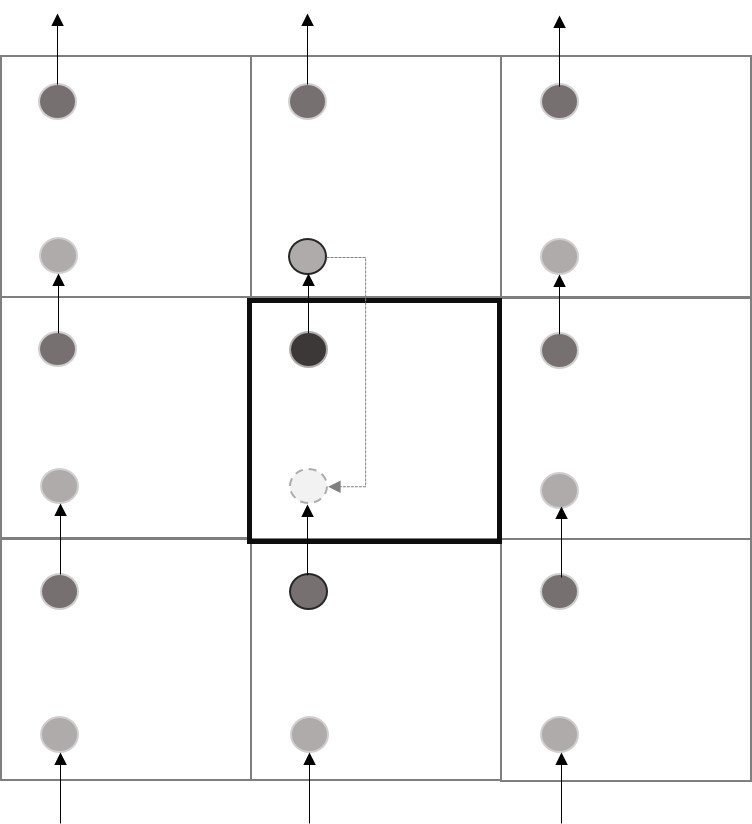
\includegraphics[scale=0.29]{imagen_min.jpg}
	\caption{Representación de la convención de imagen mínima para una lattice 2D.}
	\label{fig:min2d}
\end{figure}

 \begin{figure}[h!]
	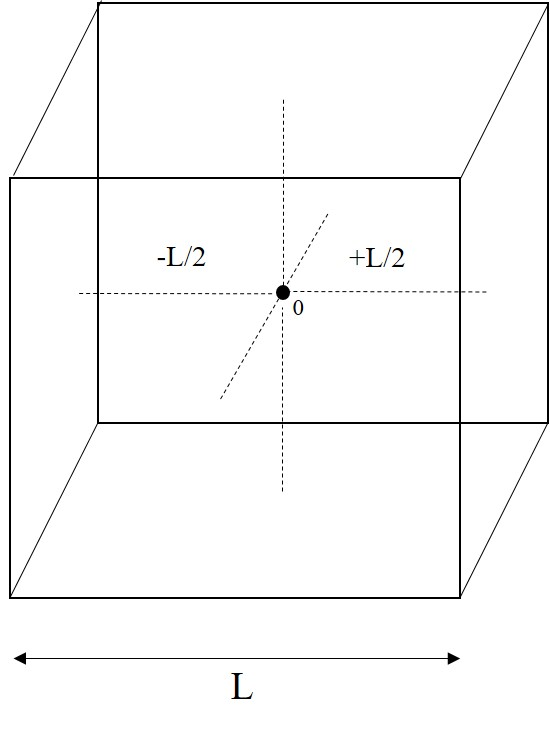
\includegraphics[scale=0.32]{imagen_min_3d.jpg}
	\caption{Celda de simulación 3D centrada en el origen de coordenadas.}
	\label{fig:min3d}
\end{figure}

\subsection{Paralelización MPI}

Para paralelizar la subrutina haremos la inicialización y finalización de MPI en el código principal incluyendo el módulo `mpif.h', y repartiremos el número de partículas según el número de procesadores que empleemos, con los vectores ini y fin. Haciendo que, si no hay un número entero de partículas, el último procesador haga una partícula de más. 
Entonces en la subrutina, los diferentes workers con un MPI$\_$ISEND enviarán sus posiciones ya modificadas de las partículas que les pertenecen al master (procesador 0). El master con un MPI$\_$RECV recibirá toda la información actualizada y enviará toda esta con un MPI$\_$ISEND a todos los workers. Estos también la recibirán con MPI$\_$RECV, consiguiendo así que todos dispongan de las nuevas posiciones ya modificadas.

Entre estos procesos de comunicación entre procesadores encontraremos llamadas a las subrutinas del módulo mpi que crean las barreras, MPI$\_$BARRIER. Estas obligan a esperar a tener toda la información de todos los workers o master antes del siguiente proceso de comunicación. 

Para ver el efecto de la paralelización de dicha subrutina se ha graficado el tiempo que tarda esta con un número concreto de partículas (N=10000 y N=100) variando el número de procesadores empleados, obteniendo,


 \begin{figure}[h!]
	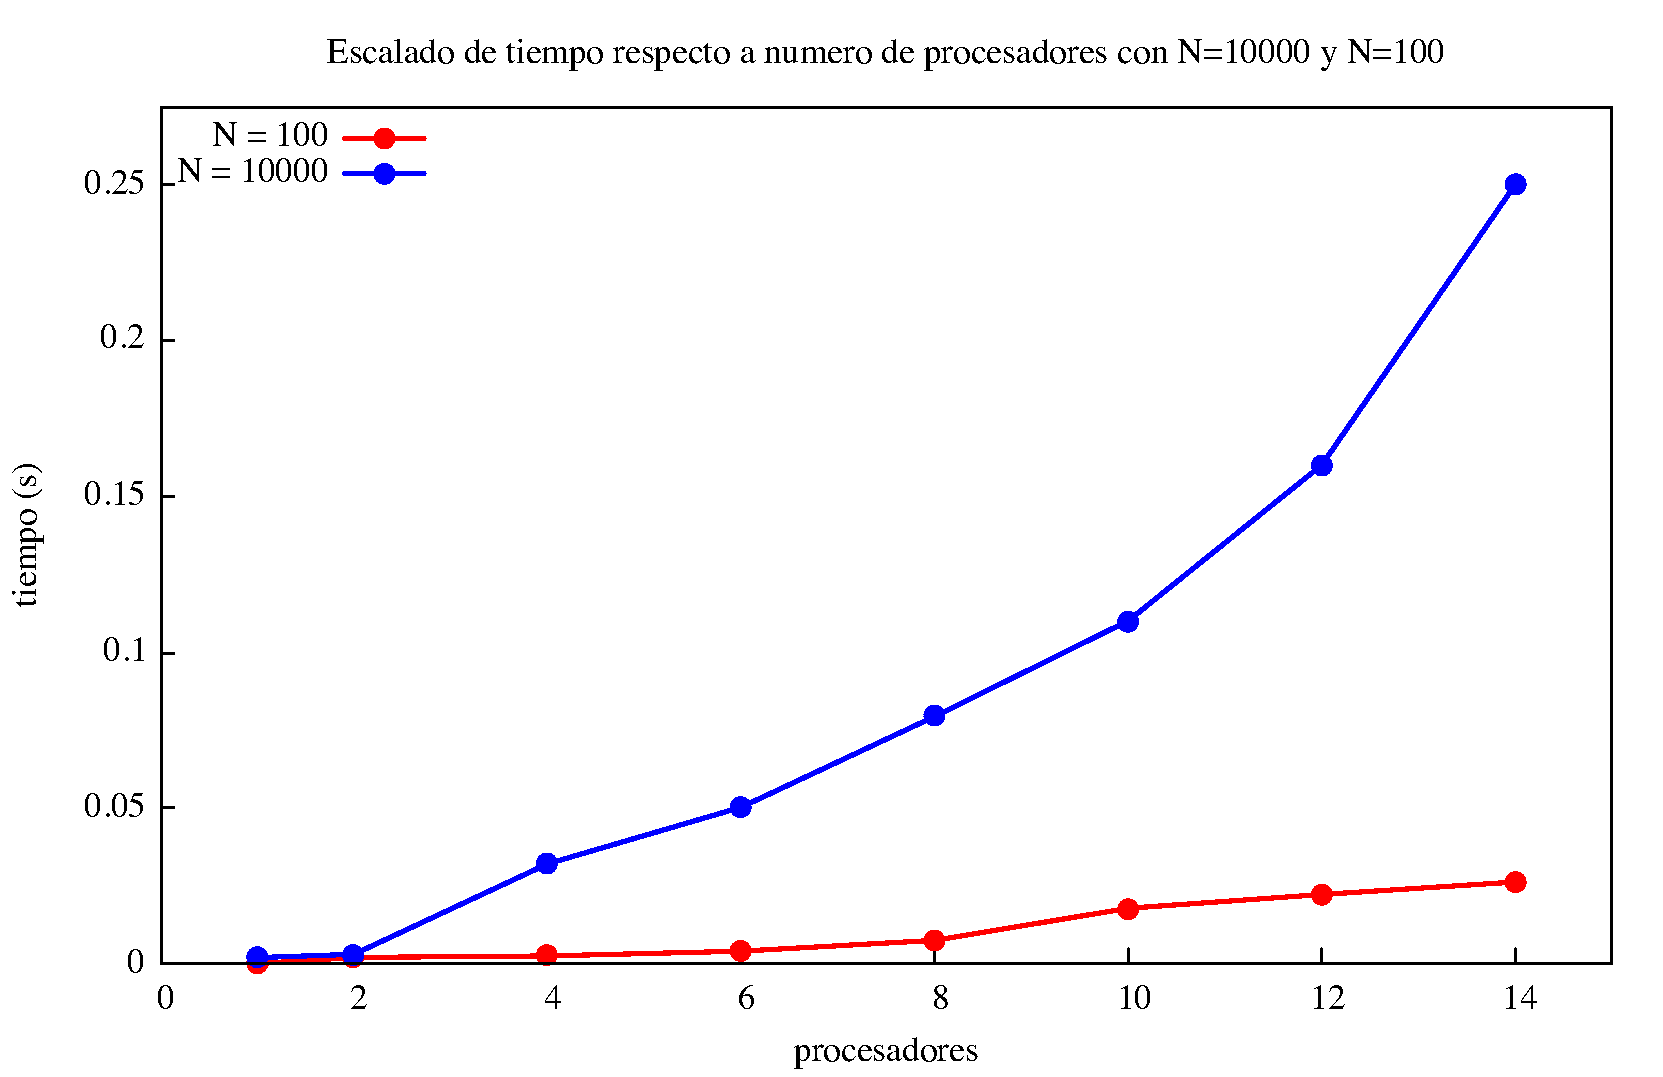
\includegraphics[scale=0.4]{lorena_proc.pdf}
	\caption{Dependencia del tiempo de ejecución de las condiciones periódicas de contorno con el número de procesadores a un número de partículas constante.}
\end{figure}


Se puede observar que en este caso particular tarda más cuanto más procesadores haya. Esto es porque lo que ralentiza el proceso no es la línea de código de condiciones periódicas, si no el proceso de comunicación entre procesadores. Observaríamos, la ley de Amdahl’s pero a la inversa con N=10000. Este efecto se observa con mayor número de partículas. En este caso, no aumenta el tiempo linealmente con el número de procesadores porque siempre tenemos una parte serial de código. 

También se ha estudiado como varia el tiempo de cálculo en función del número de partículas manteniendo un número de procesadores constante (procesadores=4). 

 \begin{figure}[h!]
	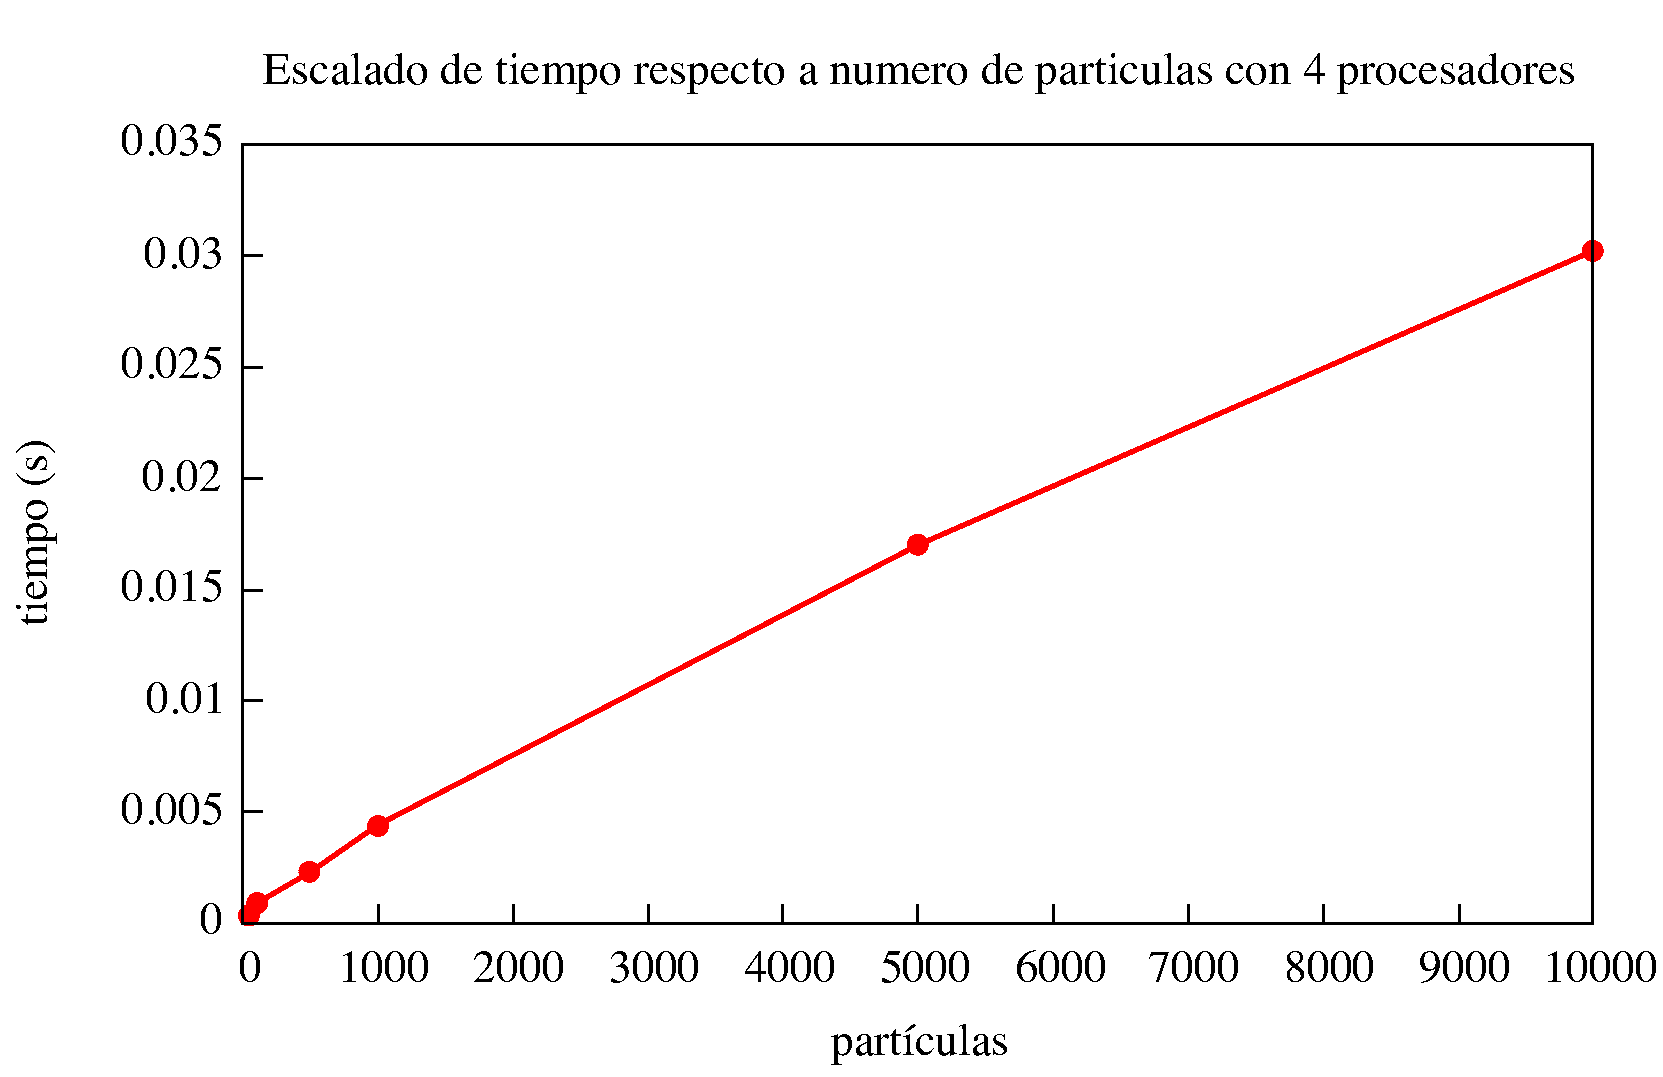
\includegraphics[scale=0.4]{lorena_particulas.pdf}
	\caption{Dependencia del tiempo de ejecución de las condiciones periódicas de contorno con el número de partículas a un número de procesadores constante.}
\end{figure}

Como es lógico a mayor número de partículas se observa un mayor tiempo de cálculo. Y se observa una tendencia aceptablemente lineal.

La determinación de puntos en ambas gráficas son resultado del promedio de diferentes medidas del tiempo ya que el clúster utilizado presenta distintos nodos, no pudiéndose controlar a cuál de ellos envía. De este modo, el resultado no es reproducible de una ejecución a otra.




\section{Data}



\section{Desplazamiento cuadrático medio}

A continuación se detallará el procedimiento seguido en la implementación de la paralelización del código de análisis visual, última parte del código de dinámica molecular desarrollado.

Para esta parte se decide calcular el desplazamiento cuadrático medio (MSD) de las partículas a lo largo de la simulación, con la expresión:
\begin{equation}\label{eq: expresion msd alberto}
MSD \equiv \langle\left(x(t)-x_{o}\right)^{2}\rangle
\end{equation}

Para calcular dicha expresión, se introduce en el archivo de entrada un valor de la frecuencia de escritura de las posiciones de las partículas (\it{restart}) y en el  \it{main} del archivo que las contiene (con el mismo nombre y extensión \it{rst}). Del mismo modo, al iniciar la simulación se determina el número de frames que contendrá el archivo de restart.

Una vez finalizada la simulación, previamente a finalizar el entorno MPI, se llama a la subrutina \it{postvisual} con la entrada de número de frames, número de partículas y dimensión del sistema.

La subrutina (en serie y en paralelo) lee el archivo generado a lo largo de la dinámica molecular en una matriz. Posteriormente, mide para cada partícula el MSD a cada frame impreso. Es decir, para una misma partícula conociendo el número de frames y partículas del sistema recorre la matriz calculando la expresión \eqref{eq: expresion msd alberto}. Dichos valores se van imprimiendo en una nueva matriz con F filas (correspondientes una a cada tiempo) y C columnas (una por cada partícula).

Finalmente, el resultado se imprime en un archivo con nombre \it{desplazamientos.dat}.

\subsection{Implementación en paralelo}
Se decide que la paralelización de la rutina se realice dividiendo las N partículas del sistema en los diferentes procesadores a usar. De este modo, se consigue que cada procesador pueda calcular el valor de MSD con la rutina ya generada para las partículas asignadas de manera autónoma, y sólo deba comunicarse con los demás al finalizar el cálculo.

Por otra parte, la lectura del archivo \it{restart.rst} se realiza también en paralelo. Éste hecho se debe a que en un primer momento se realizaba de manera única a través del MASTER y éste enviaba a cada procesador el rango correspondiente --según la división de partículas realizada-- de la matriz de entrada para que realizara el cálculo. Se observaron problemas de comunicación por parte del MASTER a los procesadores y se decidió implementar también la lectura en paralelo.

Con la lectura en paralelo se han observado los siguientes resultados:
\begin{itemize}
\item Desaparición de los problemas de comunicación existentes, al no tener que comunicarse el MASTER con cada procesador.
\item Tiempo de cálculo similar en ambos métodos, ya que la lectura del archivo se debía realizar de todos modos.
\end{itemize}
Se debe considerar que pese a que el tiempo de cálculo no aumenta, el gasto de memoria sí que incrementa debido a que la lectura del archivo \it{restart.rst} es realizada por todos los procesadores. En cualquier caso, se hace un balance positivo ya que en el método anterior intentado se habían producido problemas en algunos tests realizados a nivel de comunicación que no se habían podido solucionar.

Posteriormente, cada procesador calcula el MSD para las partículas asignadas en la división de trabajo realizada y mandan los rangos de la matriz de desplazamientos a MASTER. Éste, después de recibir los datos, los imprime en el archivo de resultados final.

Así, el proceso se puede resumir como:
\begin{enumerate}
\item Lectura del archivo de entrada completo en paralelo.
\item Cálculo del MSD en paralelo, con división por partículas en los diferentes procesadores.
\item Envío de valores de MSD de los diferentes procesadores a MASTER.
\item Impresión de los resultados en \it{desplazamientos.dat}.
\end{enumerate}

\subsection{Análisis de la implementación en paralelo}
La implementación en paralelo se ha realizado de manera satisfactoria obteniendo unos resultados de disiminución de tiempo considerables en aumentar el número de procesadores.

Para diferente número de partículas (figura \ref{fig: comparacion cores alberto} se ha analizado el tiempo de cálculo de la rutina para un número creciente de procesadores (de 1 --en serie-- a 14) observando como la disminución del tiempo de cálculo es considerable entre 2 y 6 procesadores, pero a partir de éstos el tiempo es muy parecido.
\begin{figure}
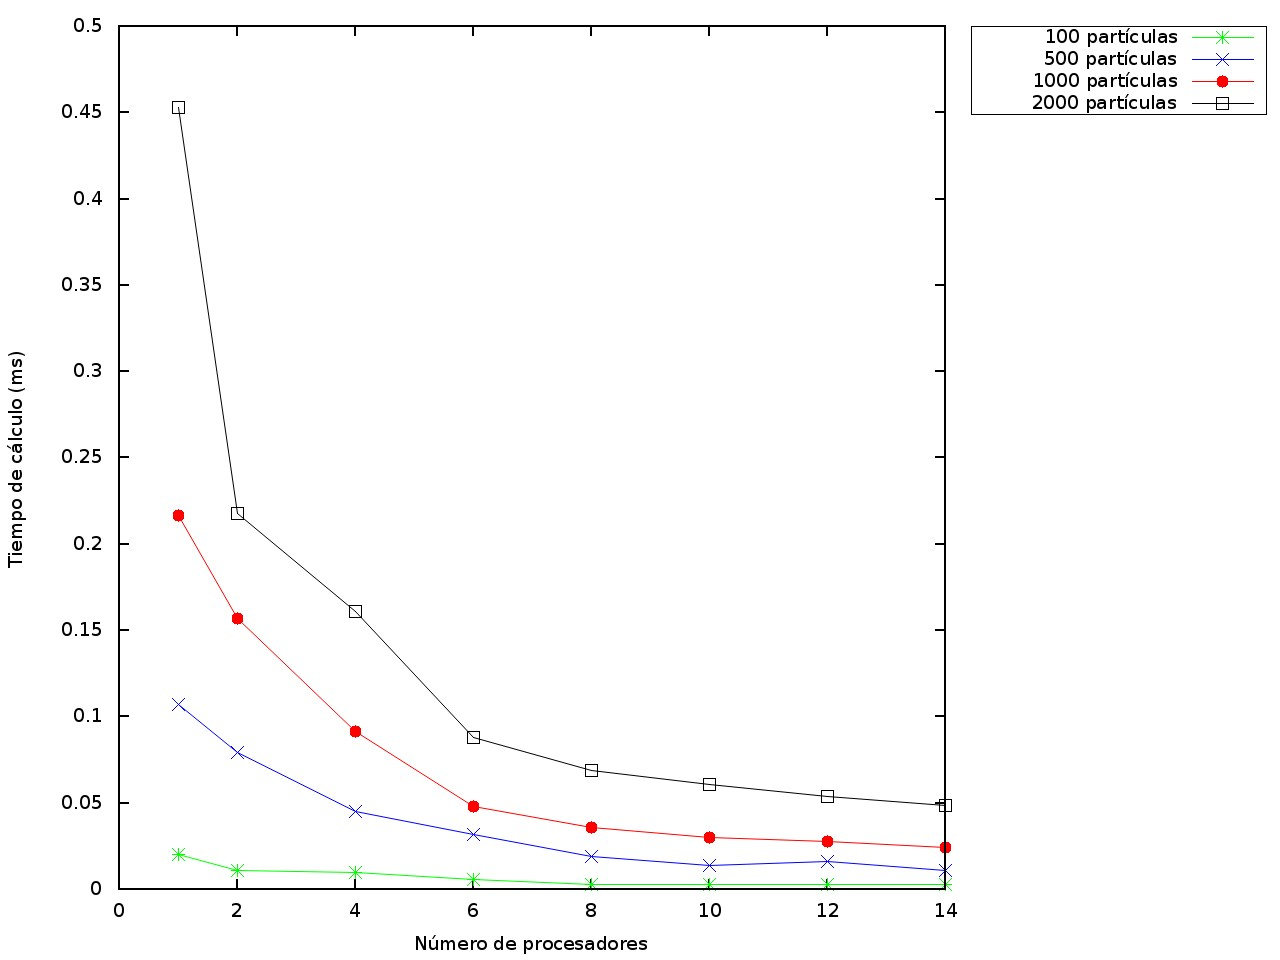
\includegraphics[scale=0.25]{velos_calc_alberto.jpeg} 
\caption{Tiempo de cálculo (ms) para diferentes sistemas (N=100,\ 500,\ 1000,\ 2000) en función de los procesadores utilizados.} 
\label{fig: comparacion cores alberto}
\end{figure}

Se puede observar como para sistemas de mayor tamaño (N=1000,2000) la disminución de velocidad entre el cálculo en serie y con dos procesadores es remarcable. Prácticamente, con 2000 partículas en aumentar el número de procesadores en dos se consiguen tiempos de cálculo comparables al sistema de 1000 partículas con dos procesadores menos. A partir de 8 procesadores dicha tendencia se pierde obteniendo un comportamiento asintótico.

Analizando el tiempo de cálculo para el mismo número de procesadores en aumentar el de partículas obtenemos un incremento lineal del tiempo, tal y como se puede observar en la figura \ref{fig: comparacionparticulasalberto}.
\begin{figure}[h!]
\includegraphics[scale=0.25]{8_cores_alberto.jpeg} 
\caption{Tiempo de cálculo (ms) para seis procesadores en función del tamaño del sistema.} 
\label{fig: comparacionparticulasalberto}
\end{figure}
En este caso, se puede observar una dependencia cuasi-lineal respecto el tiempo de cálculo y el tamaño del sistema.

\subsection{Conclusiones}
Del proceso de paralelización de la rutina de cálculo del desplazamiento cuadrático medio de las partículas, podemos concluir:
\begin{itemize}
\item El proceso de paralelización a través de la división por partículas permite disminuir el tiempo de cálculo de manera relevante en aumentar los procesadores utilizados, equiparando la velocidad a sistemas más pequeños para un número de procesadores menor o igual a 6.
\item Dicha disminución del tiempo de cálculo no se observa para un número de procesadores mayor a 6, ya que se observa un comportamiento asintótico.
\item Para un mismo número de procesadores, hay una relación cuasi-lineal entre el tiempo de cálculo y el tamaño del sistema.
\item La paralelización, pues, es efectiva para pocos procesadores y permite calcular sistemas 4 veces mayores en el mismo tiempo (veáse figura \ref{fig: comparacion cores alberto}, la velocidad para el sistema con 2000 partículas con 6 procesadores es similar al cálculo en serie con 500 partículas). 
\end{itemize}
\end{document}
